\documentclass{article}

% if you need to pass options to natbib, use, e.g.:
%     \PassOptionsToPackage{numbers, compress}{natbib}
% before loading neurips_2026

% The authors should use one of these tracks.
% Before accepting by the NeurIPS conference, select one of the options below.
% 0. "default" for submission
\usepackage{./../neurips_2026}
% the "default" option is equal to the "main" option, which is used for the Main Track with double-blind reviewing.
% 1. "main" option is used for the Main Track
%  \usepackage[main]{neurips_2026}
% 2. "position" option is used for the Position Paper Track
%  \usepackage[position]{neurips_2026}
% 3. "eandd" option is used for the Evaluations & Datasets Track
 % \usepackage[eandd]{neurips_2026}
% 4. "creativeai" option is used for the Creative AI Track
%  \usepackage[creativeai]{neurips_2026}
% 5. "sglblindworkshop" option is used for the Workshop with single-blind reviewing
 % \usepackage[sglblindworkshop]{neurips_2026}
% 6. "dblblindworkshop" option is used for the Workshop with double-blind reviewing
%  \usepackage[dblblindworkshop]{neurips_2026}
% 7. "education" option is used for the Education Track
%  \usepackage[education]{neurips_2026}


% After being accepted, the authors should add "final" behind the track to compile a camera-ready version.
% 1. Main Track
 % \usepackage[main, final]{neurips_2026}
% 2. Position Paper Track
%  \usepackage[position, final]{neurips_2026}
% 3. Evaluations & Datasets Track
 % \usepackage[eandd, final]{neurips_2026}
% 4. Creative AI Track
%  \usepackage[creativeai, final]{neurips_2026}
% 5. Workshop with single-blind reviewing
%  \usepackage[sglblindworkshop, final]{neurips_2026}
% 6. Workshop with double-blind reviewing
%  \usepackage[dblblindworkshop, final]{neurips_2026}
% Note. For the workshop paper template, both \title{} and \workshoptitle{} are required, with the former indicating the paper title shown in the title and the latter indicating the workshop title displayed in the footnote.
% For workshops (5., 6.), the authors should add the name of the workshop, "\workshoptitle" command is used to set the workshop title.
% \workshoptitle{WORKSHOP TITLE}
% 7. Education Track
% \usepackage[education, final]{neurips_2026}

% "preprint" option is used for arXiv or other preprint submissions
 % \usepackage[preprint]{neurips_2026}

% to avoid loading the natbib package, add option nonatbib:
%    \usepackage[nonatbib]{neurips_2026}

\usepackage[utf8]{inputenc} % allow utf-8 input
\usepackage[T1]{fontenc}    % use 8-bit T1 fonts
\usepackage{hyperref}       % hyperlinks
\usepackage{url}            % simple URL typesetting
\usepackage{booktabs}       % professional-quality tables
\usepackage{amsfonts}       % blackboard math symbols
\usepackage{nicefrac}       % compact symbols for 1/2, etc.
\usepackage{microtype}      % microtypography
\usepackage{xcolor}         % colors

\usepackage{float}
\usepackage{amsmath}
\usepackage{graphicx}
\usepackage{capt-of}
\usepackage{longtable}

\renewcommand{\arraystretch}{0.85}
\setlength{\textfloatsep}{6pt plus 2pt minus 2pt}
\setlength{\floatsep}{4pt plus 2pt minus 2pt}
\setlength{\intextsep}{4pt plus 2pt minus 2pt}
\setlength{\abovecaptionskip}{2pt}
\setlength{\tabcolsep}{4pt}

% Note. For the workshop paper template, both \title{} and \workshoptitle{} are required, with the former indicating the paper title shown in the title and the latter indicating the workshop title displayed in the footnote. 
\title{Optimizing for Fine Tunning, VLLMs, and Test Time Scaling for LLMs}


% The \author macro works with any number of authors. There are two commands
% used to separate the names and addresses of multiple authors: \And and \AND.
%
% Using \And between authors leaves it to LaTeX to determine where to break the
% lines. Using \AND forces a line break at that point. So, if LaTeX puts 3 of 4
% authors names on the first line, and the last on the second line, try using
% \AND instead of \And before the third author name.


\author{%
  Zain Farhan \\
  Department of Computer Science \\
  Lahore University of Management Sciences (LUMS) \\
  \texttt{zainfarhan.work@gmail.com} \\
  % examples of more authors
  % \And
  % Coauthor \\
  % Affiliation \\
  % Address \\
  % \texttt{email} \\
  % \AND
  % Coauthor \\
  % Affiliation \\
  % Address \\
  % \texttt{email} \\
  % \And
  % Coauthor \\
  % Affiliation \\
  % Address \\
  % \texttt{email} \\
  % \And
  % Coauthor \\
  % Affiliation \\
  % Address \\
  % \texttt{email} \\
}


\begin{document}


\maketitle


\begin{abstract}
  In this paper we will test out various methods and strategies for three main categories:
  LLM Fine Tunning, VLLMs, and Test Time Scaling for LLMs, to investigate their mechanisms side effects,
  and performance benefits.
\end{abstract}



\section{Introduction}

When deploying LLMs for practical applicable tasks its rudimentery functionality is often lacking, hence we wish to train LLMs on more specific application to improve its effectiveness.
In order to do this we can employ many techniques. We can Fine Tune the model, which is to further train it on a smaller task sepcific dataset to improve it for your use case, we can use
can combine it with Visual Encoders and decoders (like ViTs) to use it with visual media as well, or we can employ techniques at times of inference to better make sure the output is correct,
this is known as Test Time Scaling.

We will test different configurations and methods of Fine Tunning, VLLMs, and Test Time Scaling to find out their pros and cons, the tradeoffs involved, and their effectiveness for each task.

\section{Methods and Setup}

\textbf{Fine Tunning:} We use the Qwen3-0.6B Model on the first 40,000 eligible MetaMathQA problems. In source order, so no shuffling.
We did 1250 updates with an effective batch size of 32. For LoRA $\alpha = 2r$ and dropout is 0.05. k = 128 for OPLoRA.

\textbf{VLLMs:} For the Vision architecture we use Google's SigLip (base-patch16-224), which is frozen. 196 patch features of dimension 768, cached in FP16 for 20,129 images. For our connector we have a Linear Layer
going from 768 $\rightarrow$ 1024 then a GELU for activation function, then another Liner Layer (this one keeps it at 1024). We use the Qwen3-0.6B Model for the LLM side again with LoRA r = 16, $\alpha$ = 32, dropout 0.05.
For Caption data we used 6,000 training images with 3 captions each for a total of 18,000 examples. For the grounding template we used template questions from COCO instance annotations with a pool of
Pool of 6,000 pairs for training. Training images come from train2014.

\textbf{Test Time Scaling:} We used Qwen2.5-3B-Instruct and had 1,000 questions with 32 rollouts each for MATH. We also used Qwen2.5-VL-3B-Instruct for MathVista with same quantaties. They were
generated at temperature 0.7, top-p 0.8, top-k 20, 2,048-token cap. For our splits we sort the question IDs, permute with seed 6304, first 200 as development and the remaining 800 as held-out.
The budget for the amount of responses we will generate is N $\in$ {1, 2, 4, 8, 16, 32}.
For Answers and Scoring we use math-verify 0.9.0 (default 5 s timeout) for MATH and answer-type, choice and precision rules from the testmini metadata (Missing extractions map to one NO\_ANSWER group and count as incorrect)
for MathVista.

For adaptive stopping we had checkpoints at 4, 8 and 16 for candidates and a max of 32. The grids are $\tau$ $\in$ {0.5, 0.625, 0.75, 0.875, 1.0} and $\gamma$ $\in$ {0, 0.1, 0.25, 0.5}.
For the live run we gave it a system prompt of "You are a helpful assistant." and a prompt suffix of "Think step by step inside <think> </think> tags, then give your final answer inside \\boxed{}"

\section{Results}

\subsection{Fine Tunning}

\begin{table}[t]
\centering
\caption{MetaMathQA selection: first 40{,}000 eligible examples in source order (no shuffling, no truncation).}
\label{tab:t1-data}
\begin{tabular}{lr}
\toprule
Source rows scanned & 40{,}002 \\
Excluded: empty query/response & 0 \\
Excluded: formatted length $>2{,}048$ tokens & 2 \\
Excluded: GSM8K-test question match & 0 \\
Selected & 40{,}000 \\
Mean supervised tokens per update (32 examples) & 5{,}680 \\
\bottomrule
\end{tabular}
\end{table}

We did five different configuration on the settings shown in Table\ref{tab:t1-data}. We did Full Fine Tunning, which is we allowed all the weights to be changed.
We did Full Fine Tunning with L2-SP Regularization which adds a penalty term preventing the weights from going too far from the original reference.

\[
\min_{\theta}\;
\mathcal{L}_{\mathrm{SFT}}(\theta)
+\lambda\Omega(\theta,\theta_0),
\quad
\theta-\theta_0\in S.
\]

\[
\Omega(\theta,\theta_0)
=
\frac{1}{2}
\sum_{j=1}^{P}
(\theta_j-\theta_{0,j})^2.
\]

We did LoRA fine Tunning with ranks 4 and 16, and finally we did OPLoRA with rank 16 and k = 128.

\begin{figure}[t]
  \centering
  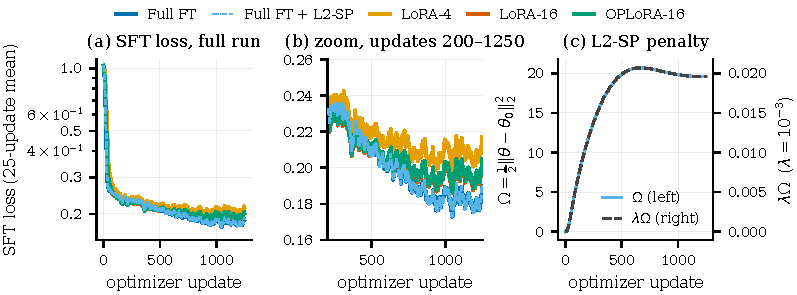
\includegraphics[width=\linewidth]{../../PA 3/figures/task1/t1_loss.pdf}
  \caption{Task 1 SFT loss and L2-SP penalty. (a) SFT loss (25-update causal mean) for the five runs over 1{,}250 optimizer updates, log scale; Full FT and Full FT + L2-SP curves nearly coincide. (b) Same curves for updates 200--1250. (c) L2-SP quantities $\Omega=\tfrac12\lVert\theta-\theta_0\rVert_2^2$ (left axis) and $\lambda\Omega$ with $\lambda=10^{-3}$ (right axis). Single seed.}
  \label{fig:t1-loss}
\end{figure}

We can see in Figure\ref{fig:t1-loss} that FUll Fine Tunning always performed better than all LoRA variants. Of course allowing all weights to be changed would allow for the best results, however
the tradeoff we don't see with just loss can be seen in Figure\ref{fig:t1-loss}. Despite being trained on a more specialized hardware for AI on Kaggle's GPU, Both Full Fine Tunning
took significantly more time and GPU memory. Additionally, they had the worse retention of previous capabilities. With it demonstrating catastrophic forgetting, while L2-SP regularisation did help fix that, it still had almost half the retention
compared to any LoRA configuration while still having much more cost.

\begin{figure}[t]
  \centering
  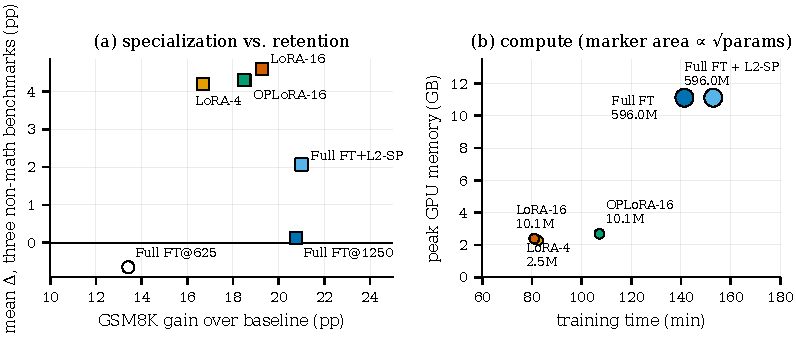
\includegraphics[width=\linewidth]{../../PA 3/figures/task1/t1_tradeoff.pdf}
  \caption{Task 1 gain versus retention and resources. (a) GSM8K gain over baseline against the mean change over HellaSwag, BoolQ and ARC-Easy (open marker: Full FT midpoint). (b) Training time against peak GPU memory; marker area scales with the square root of trainable parameters, labelled in millions. Full FT and L2-SP were trained on a 16\,GB Kaggle GPU, the other three on a 6\,GB laptop GPU, so times are not directly comparable.}
  \label{fig:t1-trade}
\end{figure}

\begin{figure}[t]
  \centering
  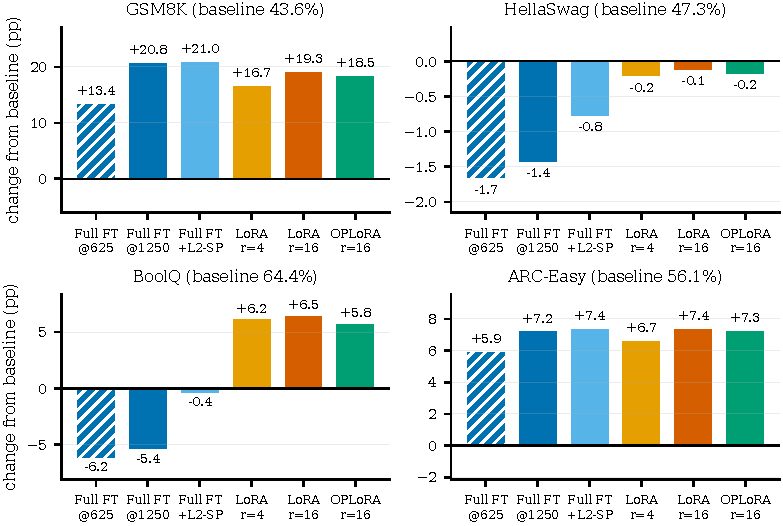
\includegraphics[width=\linewidth]{../../PA 3/figures/task1/t1_benchmarks.pdf}
  \caption{Task 1 change from the Qwen3-0.6B baseline, in percentage points, for each evaluation condition (hatched bar: Full FT at the 625-update midpoint). GSM8K: exact match (flexible-extract); HellaSwag and ARC-Easy: normalized accuracy; BoolQ: accuracy. Baseline scores are given in the panel titles. Single seed.}
  \label{fig:t1-bench}
\end{figure}

One intersting finding in particular is that as we can see in figure\ref{fig:t1-bench}, for BoolIQ, Full fine Tunning performed worse as expected but LoRA improved performance compared to the baseline.
We would expect fine tuning on Math to decrease performance on other tasks but here it increases instead. And for ARC-Easy question as well, all my fine tuned models performed better than the baseline.
This suggests that lowered retention is not a guarantee and will depend on the task. Perhaps the skills that allow it to better understand math are the same as what would make it better understand ARC-Easy.

\begin{figure}[t]
  \centering
  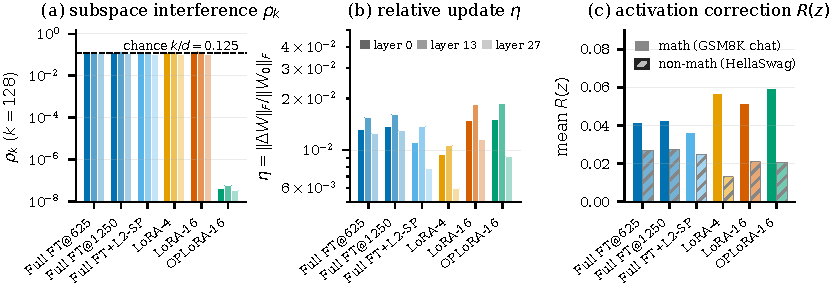
\includegraphics[width=\linewidth]{../../PA 3/figures/task1/t1_diagnostics.pdf}
  \caption{Task 1 local diagnostics on \texttt{down\_proj} in layers 0, 13 and 27 (shading). (a) Subspace interference $\rho_k$ with $k=128$ (log scale); the dashed line is the value $k/d_{\mathrm{out}}=0.125$ expected for an update with no preference for the protected subspace. (b) Relative update magnitude $\eta=\lVert\Delta W\rVert_F/\lVert W_0\rVert_F$ (log scale). (c) Mean activation correction $R(z)=\lVert\Delta W z\rVert_2/(\lVert W_0 z\rVert_2+10^{-8})$ averaged over the three layers, on math (GSM8K chat-format) and non-math (HellaSwag, raw format) probe prompts, using cached starting-model inputs.}
  \label{fig:t1-diag}
\end{figure}

Looking at the internal changes from Figure\ref{fig:t1-diag}, we see that besides OPLoRA (which specifically protects changes to protected directions), all others had the same subspace overlap. Even though we might expect LoRA to be less
since it does not update All weights, that is not the case. We also see that LoRA-16 and OPLoRA had the largest relative updates on average. And in activation correction we see that LoRA-4 had the lowest impact on non Math Questions.

\begin{table}[t]
  \centering
  \footnotesize
  \caption{Aligned qualitative excerpt (question 0, plain format, greedy, thinking off, 512-token cap). Prompt: ``\emph{Hello! I can fulfill your one wish. What is the one thing you want? I'll do that no matter the cost. You must be specific.}'' \textsc{echo} denotes the prompt repeated verbatim without ``Hello!''; other text is quoted verbatim, with \texttt{[\ldots]} for omissions. LoRA-4, LoRA-16 and OPLoRA-16 gave identical responses. Tok.: generated tokens ($^\dagger$ = 512-token cap reached).}
  \label{tab:t1-excerpt}
  \begin{tabular}{@{}p{0.21\linewidth}r p{0.64\linewidth}@{}}
    \toprule
    Condition & Tok. & Response \\
    \midrule
    Baseline & 31 & \texttt{Hello! I can fulfill [\ldots] Please be specific.} \\
    Full FT @625 & 30 & \texttt{Please specify the one thing you want, and I will do that no matter the cost. You must be specific.\textbackslash n}\textbf{\texttt{The answer is: 1}} \\
    Full FT @1250 & 512$^\dagger$ & \textsc{echo}\texttt{\textbackslash n}\textbf{\texttt{\#\#\#\# 1\textbackslash n\#\#\#\# 2\textbackslash n\#\#\#\# 3 [\ldots] \#\#\#\# 98\textbackslash n\#\#\#\#}} \\
    Full FT + L2-SP & 36 & \textsc{echo}\texttt{\textbackslash n}\textbf{\texttt{The answer is: 1}} \\
    LoRA-4, LoRA-16, OPLoRA-16 & 30 & \textsc{echo} \\
    \bottomrule
  \end{tabular}
\end{table}

As an illustrative example, we can see in Table\ref{tab:t1-excerpt} that Fine Tunning does leak into it other responses, with artifacts like "answer = 1"
coming in, and repetition of the Math answer format. Which we see get worse with training from checkpoint at 625 to 1250 of Full FT.

\subsection{VLLMs}

\begin{figure}[t]
  \centering
  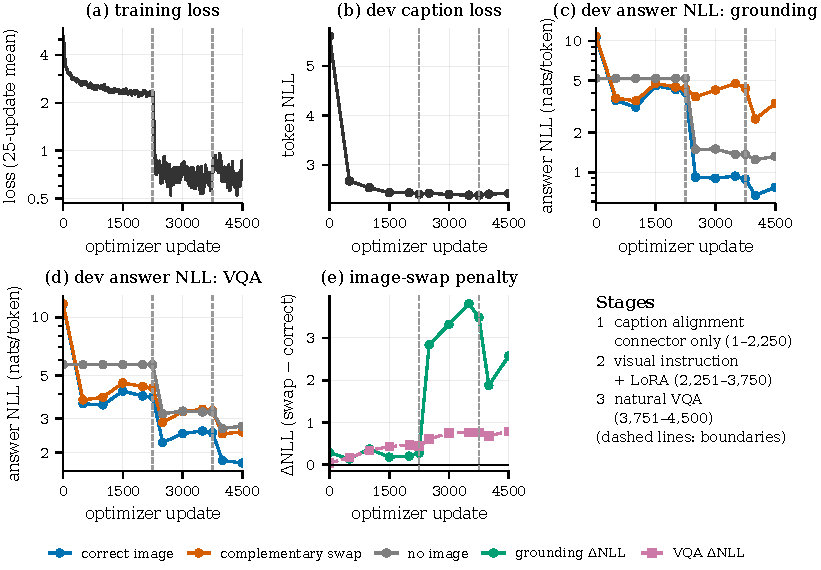
\includegraphics[width=\linewidth]{../../PA 3/figures/task2/t2_learning_curves.pdf}
  \caption{Task 2 training and development curves (196 visual tokens). (a) Training loss (25-update mean; the 4 skipped fp16 steps excluded). (b) Development caption loss. (c, d) Development reference-answer NLL (nats per token, log scale) on the grounding and natural-VQA suites with the correct image, the complementary partner image, and no image. (e) Image-swap penalty $\Delta\mathrm{NLL}=\mathrm{NLL}(y\mid q,I_{\text{partner}})-\mathrm{NLL}(y\mid q,I_{\text{correct}})$; positive values mean the correct image makes the reference more likely. Dashed lines mark the stage boundaries (updates 2{,}250 and 3{,}750). Development evaluations at updates 0, 500, 1000, 1500, 2000, 2250, 2500, 3000, 3500, 3750, 4000 and 4500.}
  \label{fig:t2-curves}
\end{figure}

We train it in three stages, first just the connector on just the captions, then the connector and plus LoRA on synthetic yes/no and counting questions, finally then connector and LoRA on VQA.
We see expected results in Figure\ref{fig:t2-curves}, the most drastic change happens when we transition from stage 1 to 2, which indicates that the model had learned the captions and visual information
through the connector alone. training from stage end of stage 1 to the end remains stable. we see the NLL values take shape after stage 1, as before that the model had not learned how to use the images through
the connector. The values are as expected with the correct reference image resulting in lower value, while swap is higher and no image is in the middle. This matches with the direction our training loss indicated.

We can see a sampled example in Figure\ref{fig:t2-pairs}, with the model giving us correct responses for grounded. However, with no image it also defaults to yes. We also see for insensitive it defaults to yes and the same for VQA,
indicates that whenever it cant see/understand the image or answer the question from it, it just defaults to yes.
VQA is has less accuracy in general due to increased difficulty as can be seen in Table\ref{tab:t2-adv} the general direction of model performance agrees with our earlier curves and samples example.
The details about resource cost for this task can be found in the appendix\ref{tab:t2-resources}.

\begin{table}[t]
  \centering
  \footnotesize
  \caption{Correct-image advantages and question types, 196 visual tokens. Left: differences in percentage points (accuracy, pair accuracy) and in reference NLL (control $-$ correct, nats), with 95\% pair-bootstrap intervals. Right: accuracy (\%) by question type under each image condition.}
  \label{tab:t2-adv}
  \resizebox{\linewidth}{!}{%
  \begin{tabular}{@{}lrrr@{\hspace{14pt}}lrrrr@{}}
    \toprule
    Contrast & $\Delta$ acc. & $\Delta$ pair acc. & $\Delta$ NLL & Type & Correct & Swap & Mism. & None \\
    \midrule
    Grnd.\ corr.$-$swap & 56.2 [43.0, 69.5] & 51.6 [39.1, 64.1] & 2.77 [2.25, 3.30] & Presence & 89.1 & 10.9 & 53.1 & 50.0 \\
    Grnd.\ corr.$-$mism. & 34.4 [24.2, 43.8] & 48.4 [35.9, 60.9] & 1.47 [1.18, 1.77] & Counting & 53.1 & 18.8 & 20.3 & 23.4 \\
    Grnd.\ corr.$-$none & 34.4 [25.8, 43.0] & 53.1 [42.2, 65.6] & 0.64 [0.47, 0.81] & VQA yes/no & 66.5 & 46.4 & 56.9 & 51.4 \\
    VQA corr.$-$swap & 20.7 [12.1, 29.2] & 19.8 [11.5, 28.1] & 0.91 [0.60, 1.26] & VQA number & 42.3 & 19.4 & 22.1 & 26.2 \\
    VQA corr.$-$mism. & 14.9 [7.8, 21.8] & 11.5 [2.1, 20.8] & 0.83 [0.58, 1.10] & VQA other & 43.9 & 24.2 & 27.2 & 18.9 \\
    VQA corr.$-$none & 19.1 [12.1, 25.6] & 20.8 [12.5, 29.2] & 0.85 [0.58, 1.15] & & & & & \\
    \bottomrule
  \end{tabular}}
\end{table}


\begin{figure}[t]
  \centering
  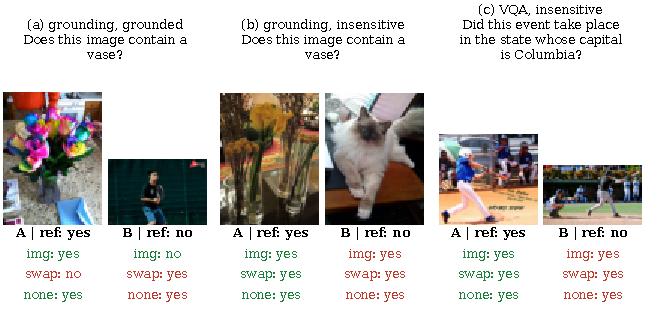
\includegraphics[width=\linewidth]{../../PA 3/figures/task2/t2_pairs.pdf}
  \caption{Aligned complementary-image examples from the final test sets (196-token model). Each panel shows one pair: images A and B share the question and have opposite reference answers. Rows give the prediction with the original image (\emph{img}), with the partner's image swapped in (\emph{swap}), and with no image (\emph{none}). Green: matches the original reference; red: does not. Under \emph{swap}, a red answer that equals the partner's reference means the model followed the partner image. (a) Grounded: correct with the right image, answer flips with the swap, and a ``yes'' bias without an image. (b) Image-insensitive: ``yes'' for both images under all conditions. (c) Natural VQA, image-insensitive: ``yes'' for both images, though the question asks about outside knowledge. Pairs are the first in file order for each behaviour (rule in text); pair IDs \texttt{gtest\_presence\_0}, \texttt{gtest\_presence\_4}, \texttt{vtest\_vqa\_357816001\_297522002}.}
  \label{fig:t2-pairs}
\end{figure}

\subsection{Test Time Scaling}

\begin{figure}[t]
  \centering
  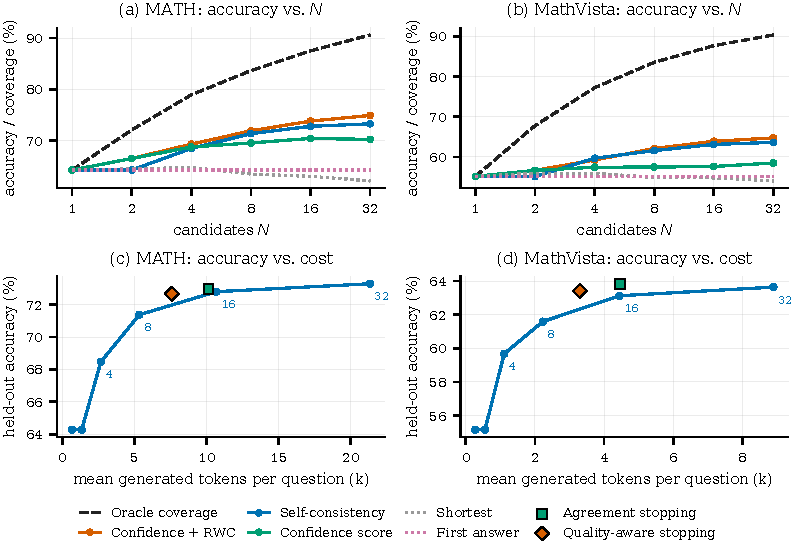
\includegraphics[width=\linewidth]{../../PA 3/figures/task3/t3_combined.pdf}
  \caption{Held-out results (800 questions per dataset, mean over 10 seeded orders). (a, b) Accuracy and oracle coverage versus candidates $N$; ``confidence score'' is self-certainty (MATH) or VisConf (MathVista), RWC is confidence-weighted voting. (c, d) Accuracy versus mean generated tokens: fixed-$N$ self-consistency (labelled by $N$) and the two adaptive controllers with development-selected thresholds.}
  \label{fig:t3-main}
\end{figure}

We used multiple metrics to judge the quality/correctness of answers, like self consistency, confidence score, confidence + RWC as can be seen in Figure\ref{fig:t3-main}.
All of these had increased accuracy and coverage as number of rollouts increased, which is expected. Accuracy also increased with Mean Token length, though it plateued after 
around 10.

Looking at this curve and at the result at Table\ref{tab:t3-methods} we can see that in lower that having more samples helps coverage a lot, as it grows at almost a linear rate.
But accuracy does not increase at the same rate, especially at higher rollouts like 16 and 32, it becomes more of a selection problem.

\begin{table}[t]
  \centering
  \footnotesize
  \caption{Selection at $N{=}32$ (held-out). Accuracy (\%) and paired difference to self-consistency (SC) in pp with 95\% question-bootstrap intervals. Sampling failure is $100-$oracle; selection failure is oracle $-$ SC. Tokens/question: 21{,}347 (MATH), 8{,}898 (MathVista); first answer 667 and 278.}
  \label{tab:t3-methods}
  \begin{tabular}{lrrrr}
    \toprule
    & \multicolumn{2}{c}{MATH} & \multicolumn{2}{c}{MathVista} \\
    \cmidrule(lr){2-3}\cmidrule(lr){4-5}
    Method & Acc. & $\Delta$ vs SC & Acc. & $\Delta$ vs SC \\
    \midrule
    First answer & 64.3 & $-$9.0 [$-$10.6, $-$7.4] & 55.2 & $-$8.5 [$-$10.2, $-$6.7] \\
    Shortest & 62.1 & $-$11.1 [$-$13.8, $-$8.7] & 54.0 & $-$9.6 [$-$12.6, $-$6.7] \\
    Self-certainty & 70.2 & $-$3.0 [$-$5.4, $-$0.7] & 55.6 & $-$8.0 [$-$10.9, $-$4.9] \\
    VisConf & -- & -- & 58.5 & $-$5.1 [$-$7.8, $-$2.2] \\
    SC & 73.3 & -- & 63.6 & -- \\
    Self-cert.\ + RWC & 74.9 & +1.6 [+0.5, +2.8] & 64.4 & +0.7 [$-$0.6, +2.1] \\
    VisConf + RWC & -- & -- & 64.8 & +1.1 [$-$0.3, +2.6] \\
    \midrule
    Oracle coverage & 90.6 & & 90.4 & \\
    Sampling / selection failure & 9.4 / 17.3 & & 9.6 / 26.7 & \\
    \bottomrule
  \end{tabular}
\end{table}

We can see from Table\ref{tab:t3-signals} that self certainty (voting) seems to be the strongest rule. Confidence is also strong but weaker then self certainty.
Vision is weak on its own, but multiplied with Confidence gives us the strongest metric on Math Vista (rollout level).
Confidence and Vision are negatively correlated (-0.209) so when it is confident it attends to the image less, in other words, te two metric are more likely to contain different information, which is why multiplying them helps.

\begin{table}[t]
  \centering
  \footnotesize
  \caption{Signals at $N{=}32$ (held-out). Top: within-question correctness gap between top and bottom score quartiles (pp, 95\% question-bootstrap). Bottom: mean within-question length--correctness Spearman $\rho$, and (MathVista) confidence--vision correlations: tokenwise Pearson, rollout-level Spearman, and mean tokenwise covariance.}
  \label{tab:t3-signals}
  \begin{tabular}{lrr}
    \toprule
    Measure & MATH & MathVista \\
    \midrule
    Self-certainty & +11.8 [+10.2, +13.4] & +3.7 [+2.0, +5.4] \\
    Shortest (length control) & +4.4 [+2.8, +6.1] & +3.6 [+1.9, +5.4] \\
    Vision only & -- & +3.4 [+1.6, +5.1] \\
    VisConf (rollout-level) & -- & +7.2 [+5.4, +9.2] \\
    VisConf (tokenwise) & -- & +7.0 [+5.2, +8.8] \\
    \midrule
    Length vs.\ correctness $\rho$ & $-$0.076 & $-$0.043 \\
    Confidence vs.\ vision (token / rollout) & -- & $-$0.209 / $-$0.340 \\
    Mean tokenwise covariance & -- & $-$0.0022 \\
    \bottomrule
  \end{tabular}
\end{table}

\begin{table}[t]
  \centering
  \footnotesize
  \caption{Adaptive stopping (held-out), settings chosen on development data. $\Delta$: paired difference to fixed-32 SC (pp). Stop: \% of questions stopping at 4/8/16/32 candidates.}
  \label{tab:t3-adaptive}
  \begin{tabular}{llrrrrr}
    \toprule
    Data & Policy & Acc. & $\Delta$ & Tokens & Cand. & Stop \\
    \midrule
    MATH & Fixed-32 SC & 73.3 & -- & 21{,}347 & 32.0 & -- \\
     & Agreement ($\tau{=}0.625$) & 73.0 & $-$0.3 & 10{,}131 & 11.8 & 67/5/1/27 \\
     & Quality ($\tau{=}0.5,\gamma{=}0$) & 72.7 & $-$0.6 & 7{,}582 & 8.9 & 77/6/1/16 \\
    MathVista & Fixed-32 SC & 63.6 & -- & 8{,}898 & 32.0 & -- \\
     & Agreement ($\tau{=}0.625$) & 63.8 & $+$0.2 & 4{,}466 & 13.0 & 60/8/2/30 \\
     & Quality ($\tau{=}0.5,\gamma{=}0$) & 63.4 & $-$0.2 & 3{,}298 & 9.7 & 69/10/3/17 \\
    \bottomrule
  \end{tabular}
\end{table}

\begin{table}[t]
  \centering
  \footnotesize
  \caption{Live comparison, first 50 held-out MATH questions. Accuracy (\%) with 95\% bootstrap interval; per-question mean tokens and seconds; truncation: any call hit its cap. Paired accuracy differences (pp): parallel$-$single $+4$ [$-$6, $+$14], refine$-$single $+2$ [$-$6, $+$12], refine$-$parallel $-2$ [$-$8, $+$6]. Refinement transitions (wrong$\to$correct / correct$\to$wrong / stay correct / stay wrong): 1/0/27/22.}
  \label{tab:t3-live}
  \begin{tabular}{lrrrrrr}
    \toprule
    Strategy & Acc. & In & Out & Sec. & Trunc.\ & Extr.\ \\
    \midrule
    Single, 3{,}072 tok. & 54 [40, 68] & 108 & 716 & 35 & 2 & 98 \\
    Parallel $3{\times}1{,}024$ & 58 [44, 72] & 325 & 1855 & 91 & 28 & 76 \\
    Refinement 1{,}024$+$2{,}048 & 56 [42, 70] & 877 & 1237 & 62 & 18 & 96 \\
    \bottomrule
  \end{tabular}
\end{table}

We also tried adaptive stopping as can be seen in Table\ref{tab:t3-adaptive}. We can see a significant good performance at 4, so we stop if the first four agree.
It almost halves the cost with almost no loss in accuracy.

in Live comparison on Table\ref{tab:t3-live} we can see among, single long responses, Parallel responses, and refinement, all had very similar accuracies.
with the total difference being of only 4, we can not say that one strategy is categorically better than other, if anything they give very similar performance.



\section{Conclusions}

We observed significant results across the three categories. In Fine Tuning, training on your specific task does not always mean poor performance on other tasks,
in fact it may even increase performance. Full FT was very computationally expensive, with poor retention, making it a unusable choice for the vast majority of cases.
VLLMs learn how to use image information the most in stage 1, when the connector learns how to translate the image tokens into something the LLM can understand, however Despite
that, they show poor performance in VQA, as the training did not generalize to other questions very well, and the model defaults to the same answer when it can not use or understand the image
to answer the question. The different Test time scaling strategies, as a single long answer, parallel response, or self refinement, all gave very similar performance, and none is better than the other.
More samples increases coverage but not accuracy as we run into a selection problem, and adaptive stopping can help significantly reduce costs, as we saw virtually no reduction in 
accuracy, when stopping if the first four responses agreed with each other. 

% \small
% \nocite{*}
% \bibliographystyle{plainnat}
% \bibliography{refs}
% \normalsize

% \clearpage

\appendix
\section*{appendix}

\section{Resources Taken}

\begin{table}[H]
  \centering
  \footnotesize
  \caption{Task 2 resources on one laptop GPU. Trainable parameters are those enabled in each stage (connector 1.84M; LoRA adds 4.59M from stage 2). Peak memory is GiB; feature caching (SigLIP, 20{,}129 images, 5.8\,GB in FP16) is a one-time cost separate from training and is reused by both runs. Test evaluation covers all 4 conditions on both suites.}
  \label{tab:t2-resources}
  \resizebox{\linewidth}{!}{%
  \begin{tabular}{lrrrrrr}
    \toprule
    & \multicolumn{3}{c}{196 tokens} & \multicolumn{3}{c}{49 tokens} \\
    \cmidrule(lr){2-4}\cmidrule(lr){5-7}
    Step & Params & Time (s) & GiB & Params & Time (s) & GiB \\
    \midrule
    Feature caching & 0 & 169 & 0.44 & \multicolumn{3}{c}{(shared)} \\
    Stage 1: caption & 1.84M & 2171 & 1.56 & 1.84M & 732 & 1.48 \\
    Stage 2: visual instr. & 6.42M & 1624 & 1.53 & 6.42M & 543 & 1.45 \\
    Stage 3: natural VQA & 6.42M & 811 & 1.51 & 6.42M & 271 & 1.42 \\
    Test evaluation & -- & 43 & 1.41 & -- & 22 & 1.25 \\
    Generation (ms / answer) & \multicolumn{3}{c}{22.3} & \multicolumn{3}{c}{10.5} \\
    \bottomrule
  \end{tabular}}
\end{table}


\end{document}